\chapter{Discussion and Analysis}
\label{ch:discussion}

This chapter delves into the insights drawn from the results presented in the previous chapter, evaluating the performance of ChatGPT in generating solutions for data structures and algorithms (DSA) problems across various topics and under different prompts. The discussion aims to interpret the significance of the findings, highlight key limitations, and suggest avenues for future research.

\section{Impact of Keywords in Prompts on Acceptance Rates}
The effectiveness of the prompts in guiding ChatGPT towards successful solutions is notably influenced by specific keywords. For instance, the inclusion of the word "efficient" in Prompts 4, 6, and 9 correlated with a higher number of accepted solutions, as shown in Table~\ref{tab:accepted_solutions_per_prompt}. This suggests that directing ChatGPT to focus on efficiency not only in code execution but also in resource utilization resonates well with the model's capabilities in optimizing solutions.

\section{Role Influence on Prompt Performance}
Analysis of the role-specified in each prompt reveals a significant impact on performance. Prompts that described the user as an "expert" or "software engineer" tended to perform better, implying that a higher expectation in the role description possibly aligns better with ChatGPT's training on professional and technical language. Conversely, prompts that positioned the user as a "junior programmer" or "student" saw slightly lower acceptance rates, suggesting a mismatch between the complexity of problems and the assumed knowledge base of the role.

\section{Topic-wise Acceptance Rates}
Figure~\ref{fig:topic_wise_acceptance} presents a comparison of provided versus calculated acceptance rates across various DSA topics. The provided rates represent the expected success rates based on historical data, while the calculated rates are derived from ChatGPT's performance across nine prompts.

\begin{figure}[H]
    \centering
    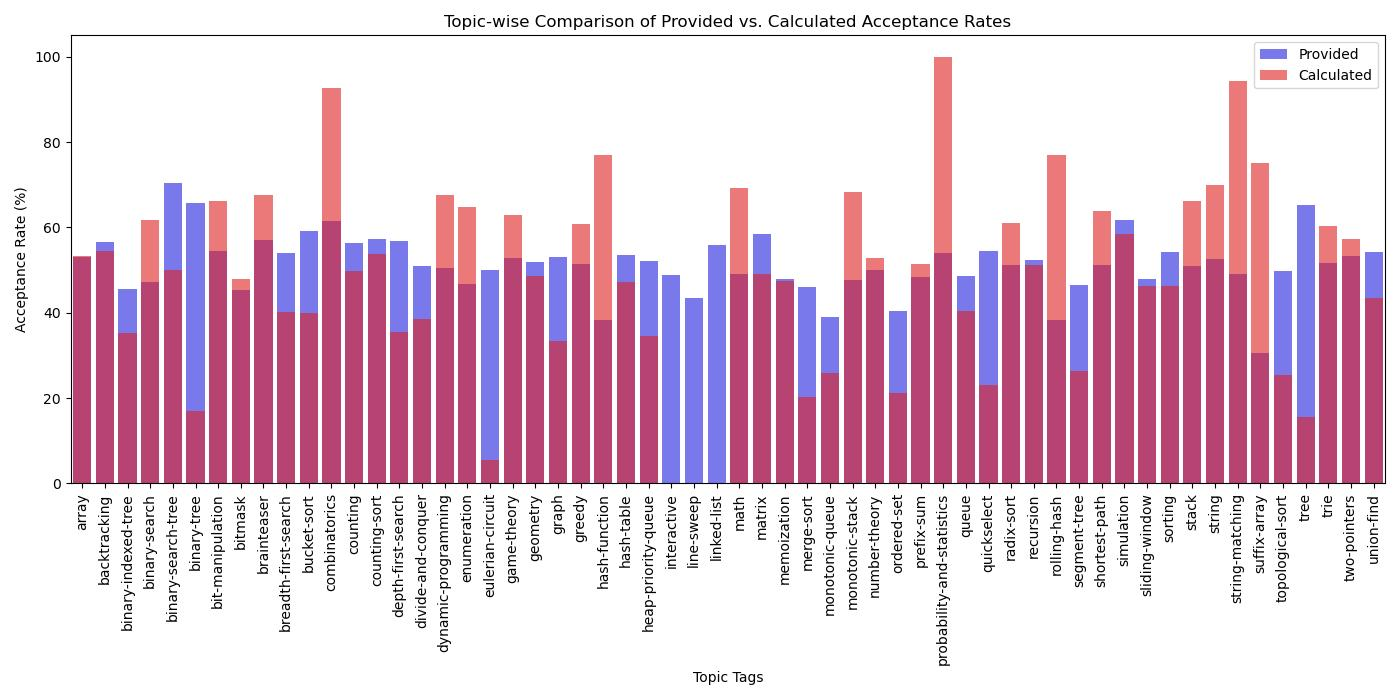
\includegraphics[width=1\textwidth]{figures/acceptance_topic_wise.jpg}
    \caption{Topic-wise comparison of provided vs. calculated acceptance rates}
    \label{fig:topic_wise_acceptance}
\end{figure}

ChatGPT exhibited exceptional performance in topics related to probability, statistics, combinatorics, hash function, rolling hash, string matching, and suffix array. These topics often involve a significant amount of mathematical reasoning and pattern recognition, areas where machine learning models like ChatGPT are particularly strong. On the other hand, the model struggled with topics such as binary tree, eulerian circuit, line sweep, linked list, and tree, which require a deep understanding of data structure manipulation and spatial relationships—a current limitation of language-based AI models.

\section{Implications of Findings}
The findings underscore the importance of prompt design in the effective utilization of AI for problem-solving in coding. By aligning the prompts with ChatGPT's training and capabilities, and by specifically targeting its strengths in mathematical reasoning and pattern recognition, the efficiency of AI-assisted coding solutions can be significantly enhanced.

\section{Limitations and Future Work}
While the study provides valuable insights into the capabilities of ChatGPT, it also highlights limitations, particularly in handling complex data structures. Future work could explore more granular prompt engineering, incorporate visual or spatial data representation techniques, and extend the analysis to newer versions of language models that might offer improved understanding of complex algorithms and data structures.

\section{Summary}
This chapter has discussed the key findings from the evaluation of ChatGPT's performance in solving DSA problems, highlighting how specific keywords and role expectations in prompts influence the effectiveness of the solutions generated. The analysis of topic-wise acceptance rates has revealed areas where ChatGPT excels and struggles, providing a roadmap for both leveraging its strengths and addressing its weaknesses in future applications.
